\documentclass[border=14pt]{standalone}
% ---------------------------------------------------------------------------
% common.tex -- shared preamble for the hand-drawn TikZ diagrams of the thesis.
%
% Every diagram in this folder is a standalone document that inputs this file.
% Change a colour or a style here and it propagates to all figures at the next
% run of ./build.sh.
% ---------------------------------------------------------------------------

\usepackage[T1]{fontenc}
\usepackage{lmodern}
\usepackage{amsmath}
\usepackage{tikz}
\usetikzlibrary{arrows.meta, positioning, fit, backgrounds, calc, shapes.geometric}

% --- palette ---------------------------------------------------------------
\definecolor{diagInk}{RGB}{38,42,50}        % text
\definecolor{diagLine}{RGB}{118,128,142}    % neutral arrows and rules
\definecolor{diagGround}{RGB}{226,233,243}  % ground-and-solve fills
\definecolor{diagGroundEdge}{RGB}{ 96,132,178}
\definecolor{diagLazy}{RGB}{225,240,228}    % lazy fills
\definecolor{diagLazyEdge}{RGB}{ 76,147,100}
\definecolor{diagNeutral}{RGB}{242,242,244} % shared machinery
\definecolor{diagNeutralEdge}{RGB}{150,155,165}
\definecolor{diagAlert}{RGB}{252,232,229}   % the expensive artefact
\definecolor{diagAlertEdge}{RGB}{198, 88, 74}

% --- styles ----------------------------------------------------------------
\tikzset{
  % generic rounded box; the colour is given by one of the *fill styles below
  box/.style={
    draw, rounded corners=2.2pt, line width=0.7pt,
    align=center, inner xsep=7pt, inner ysep=6pt,
    font=\small, text=diagInk, minimum height=9.5mm
  },
  ground/.style={box, fill=diagGround, draw=diagGroundEdge},
  lazy/.style={box, fill=diagLazy,   draw=diagLazyEdge},
  neutral/.style={box, fill=diagNeutral, draw=diagNeutralEdge},
  alert/.style={box, fill=diagAlert,  draw=diagAlertEdge},
  % a box that holds code-like text
  mono/.style={font=\small\ttfamily},
  % arrows
  flow/.style={-{Stealth[length=2.6mm,width=2.0mm]}, draw=diagLine, line width=0.8pt},
  biflow/.style={{Stealth[length=2.6mm,width=2.0mm]}-{Stealth[length=2.6mm,width=2.0mm]},
                 draw=diagLine, line width=0.8pt},
  dashflow/.style={flow, dashed, dash pattern=on 2.6pt off 2.0pt},
  % small caption-like labels
  tag/.style={font=\scriptsize, text=diagInk, inner sep=2pt},
  lane/.style={font=\small\bfseries, text=diagInk},
  % the light band that groups a lane of the diagram
  band/.style={rounded corners=3pt, draw=none, inner sep=9pt},
}


\begin{document}

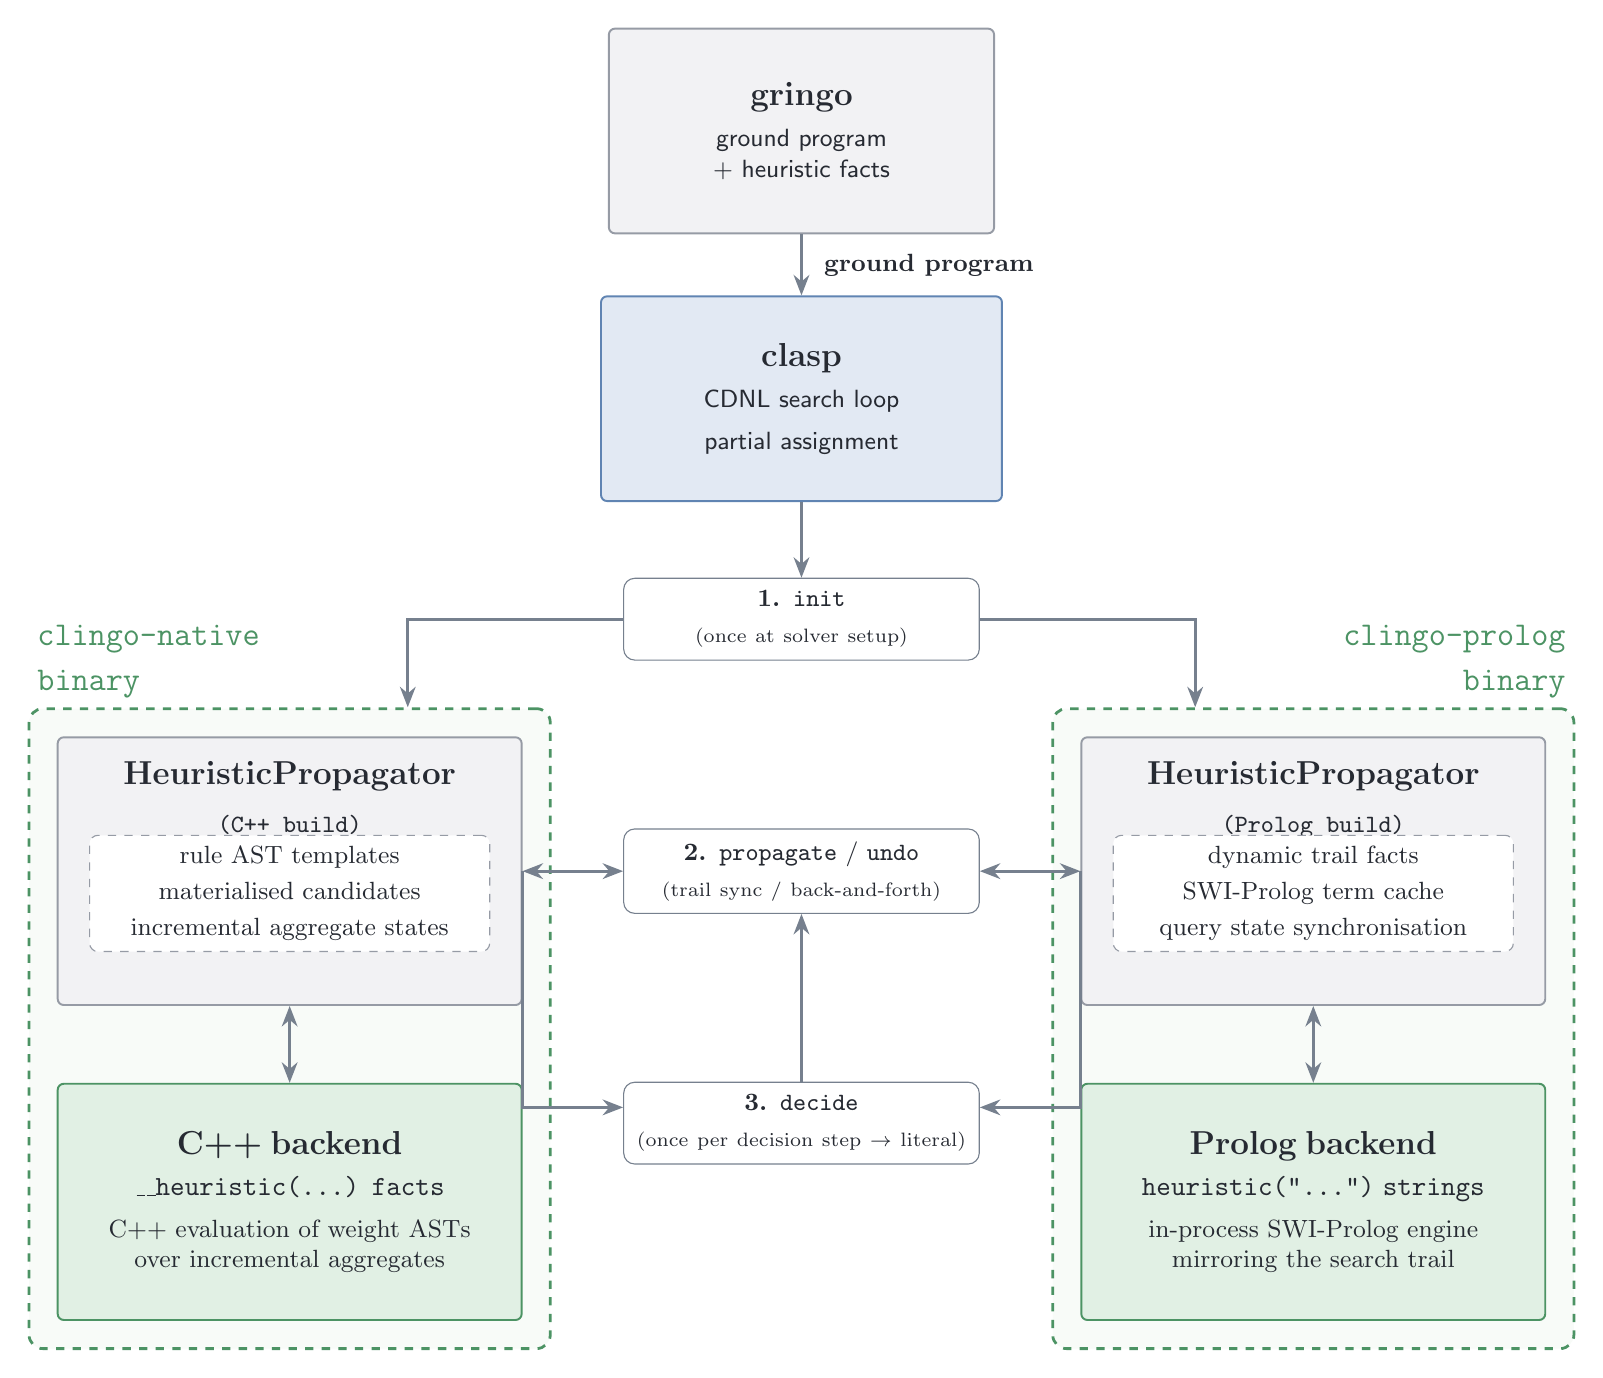
\begin{tikzpicture}

% ===========================================================================
% TOP CENTER COLUMN: Stacked gringo and clasp
% ===========================================================================
\node[neutral, text width=44mm, minimum height=26mm, align=center] (gringo) at (5.0, 9.8)
      {{\large\bfseries gringo}\\[4pt]
       {\small\sffamily ground program\\ + heuristic facts}};

\node[ground, text width=46mm, minimum height=26mm, align=center] (clasp) at (5.0, 6.4)
      {{\large\bfseries clasp}\\[4pt]
       {\small\sffamily CDNL search loop\\[4pt]
        partial assignment}};

\draw[flow, line width=1.0pt] (gringo) -- (clasp)
      node[tag, midway, right=2mm, font=\small\bfseries] {ground program};

% ===========================================================================
% BOTTOM LEFT COLUMN: clingo-native binary (HeuristicPropagator above C++ backend)
% ===========================================================================
\node[neutral, text width=54mm, minimum height=34mm] (prop_native) at (-1.5, 0.4) {};
\node[font=\large\bfseries, text=diagInk, anchor=north] (title_nat)
      at ($(prop_native.north)+(0,-2mm)$) {HeuristicPropagator};
\node[font=\small\ttfamily\bfseries, text=diagInk, anchor=north]
      at ($(title_nat.south)+(0,-0.5mm)$) {(C++ build)};

\node[draw=diagNeutralEdge, dashed, rounded corners=3pt, fill=white,
      text width=48mm, align=center, font=\small, text=diagInk,
      inner sep=4pt, anchor=north] at ($(prop_native.north)+(0,-12.5mm)$)
      {rule AST templates\\[2pt]
       materialised candidates\\[2pt]
       incremental aggregate states};

\node[lazy, text width=54mm, minimum height=30mm, align=center] (native) at (-1.5, -3.8)
      {{\large\bfseries C++ backend}\\[4pt]
       {\normalsize\ttfamily\bfseries \_\_heuristic(\dots) facts}\\[4pt]
       {\small C++ evaluation of weight ASTs\\ over incremental aggregates}};

\draw[biflow, line width=1.0pt] (prop_native) -- (native);

\begin{scope}[on background layer]
  \node[draw=diagLazyEdge, fill=diagLazy!25, dashed, rounded corners=5pt, line width=1.0pt,
        fit=(prop_native) (native), inner sep=10pt] (box_native) {};
  \node[font=\large\bfseries\ttfamily, text=diagLazyEdge, anchor=south west, align=left]
        at (box_native.north west) {clingo-native\\[2pt]binary};
\end{scope}

% ===========================================================================
% BOTTOM RIGHT COLUMN: clingo-prolog binary (HeuristicPropagator above Prolog backend)
% ===========================================================================
\node[neutral, text width=54mm, minimum height=34mm] (prop_prolog) at (11.5, 0.4) {};
\node[font=\large\bfseries, text=diagInk, anchor=north] (title_pro)
      at ($(prop_prolog.north)+(0,-2mm)$) {HeuristicPropagator};
\node[font=\small\ttfamily\bfseries, text=diagInk, anchor=north]
      at ($(title_pro.south)+(0,-0.5mm)$) {(Prolog build)};

\node[draw=diagNeutralEdge, dashed, rounded corners=3pt, fill=white,
      text width=48mm, align=center, font=\small, text=diagInk,
      inner sep=4pt, anchor=north] at ($(prop_prolog.north)+(0,-12.5mm)$)
      {dynamic trail facts\\[2pt]
       SWI-Prolog term cache\\[2pt]
       query state synchronisation};

\node[lazy, text width=54mm, minimum height=30mm, align=center] (prolog) at (11.5, -3.8)
      {{\large\bfseries Prolog backend}\\[4pt]
       {\normalsize\ttfamily\bfseries heuristic("\dots") strings}\\[4pt]
       {\small in-process SWI-Prolog engine\\ mirroring the search trail}};

\draw[biflow, line width=1.0pt] (prop_prolog) -- (prolog);

\begin{scope}[on background layer]
  \node[draw=diagLazyEdge, fill=diagLazy!25, dashed, rounded corners=5pt, line width=1.0pt,
        fit=(prop_prolog) (prolog), inner sep=10pt] (box_prolog) {};
  \node[font=\large\bfseries\ttfamily, text=diagLazyEdge, anchor=south east, align=right]
        at (box_prolog.north east) {clingo-prolog\\[2pt]binary};
\end{scope}

% ===========================================================================
% 3 SEPARATE VERTICAL CALLBACK BOXES IN THE CENTER WITH ADEQUATE ARROWS
% ===========================================================================

% --- Step 1: init (once at startup) ---
\node[fill=white, draw=diagLine, rounded corners=4pt, inner sep=4.5pt, align=center, text width=42mm, font=\small, text=diagInk]
      (box_init) at (5.0, 3.6)
      {\textbf{1. }\texttt{init}\\[2pt]{\scriptsize (once at solver setup)}};

\draw[flow, line width=1.0pt] (clasp.south) -- (box_init.north);
\draw[flow, line width=1.0pt] (box_init.west) -| ($(box_native.north)+(1.5,0)$);
\draw[flow, line width=1.0pt] (box_init.east) -| ($(box_prolog.north)+(-1.5,0)$);

% --- Step 2: propagate / undo (back-and-forth trail sync loop) ---
\node[fill=white, draw=diagLine, rounded corners=4pt, inner sep=4.5pt, align=center, text width=42mm, font=\small, text=diagInk]
      (box_prop) at (5.0, 0.4)
      {\textbf{2. }\texttt{propagate} / \texttt{undo}\\[2pt]{\scriptsize (trail sync / back-and-forth)}};

\draw[biflow, line width=1.0pt] (box_prop.west) -- (prop_native.east);
\draw[biflow, line width=1.0pt] (box_prop.east) -- (prop_prolog.west);

% --- Step 3: decide (once per decision step -> literal) ---
\node[fill=white, draw=diagLine, rounded corners=4pt, inner sep=4.5pt, align=center, text width=42mm, font=\small, text=diagInk]
      (box_decide) at (5.0, -2.8)
      {\textbf{3. }\texttt{decide}\\[2pt]{\scriptsize (once per decision step $\to$ literal)}};

\draw[flow, line width=1.0pt] (prop_native.east) |- ($(box_decide.west)+(0,2mm)$);
\draw[flow, line width=1.0pt] (prop_prolog.west) |- ($(box_decide.east)+(0,2mm)$);
\draw[flow, line width=1.0pt] (box_decide.north) -- (box_prop.south);

\end{tikzpicture}

\end{document}
